\subsubsection{Uneven Visual Spacing Scenario 2}
\begin{tikzpicture}

\foreach \x in {0,1,2,3,4}
    \draw (\x cm,0.0) -- (\x cm, 5);
    
\draw [line width=10] (0,1.175) -- (1,1.175);
\draw [line width=10] (1,2.175) -- (2,2.175);
\draw [line width=10] (2,3.175) -- (3,3.175);
\draw [line width=10] (3,4.175) -- (4,4.175);

\draw [decorate,decoration={brace,amplitude=7pt}](-0.1,1) -- (-0.1,2);
\draw [decorate,decoration={brace,amplitude=7pt}](-0.1,2) -- (-0.1,3);
\draw [decorate,decoration={brace,amplitude=7pt}](-0.1,3) -- (-0.1,4);

\foreach \x in {2,3,4}
    \draw [dotted](0,\x) -- (\x,\x);

\draw (-1, 1.5) node {1/1};
\draw (-1, 2.5) node {1/8};
\draw (-1, 3.5) node {1/4};

\draw [<-] (4.0,1) -- (4.5,1) node [anchor=west, xshift=0.5] {\textcolor{darkgreen}{0.25x}};
\draw [<-] (4.0,2) -- (4.5,2) node [anchor=west, xshift=0.5] {\textcolor{darkgreen}{2.0x}};
\draw [<-] (4.0,3) -- (4.5,3) node [anchor=west, xshift=0.5] {\textcolor{darkgreen}{1.0x}};

\end{tikzpicture}
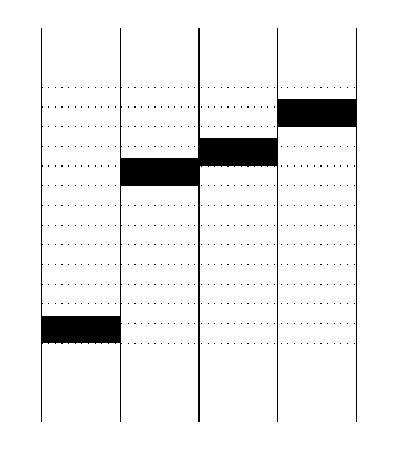
\begin{tikzpicture}

\foreach \x in {0,1,2,3,4}
    \draw (\x cm,0.0) -- (\x cm, 5);
    
\draw [line width=10] (0,1.175) -- (1,1.175);
\draw [line width=10] (1,3.175) -- (2,3.175);
\draw [line width=10] (2,3.425) -- (3,3.425);
\draw [line width=10] (3,3.925) -- (4,3.925);

\foreach \x in {4,5,6,7,8,9,10,11,12,13,14,15,16,17}
    \draw [dotted](0,0.25*\x) -- (4,0.25*\x);

\end{tikzpicture}

\noindent
\textbf{Gameplay View} (left) vs. \textbf{Editor View (Scale: 0.5)} (right)\newline
\textit{Each dotted line in Editor View represents} $1/8$
